\documentclass[11pt]{article}

% ---------- Packages ----------
\usepackage[a4paper,margin=1in]{geometry}
\usepackage{amsmath,amssymb,amsthm,mathtools}
\usepackage{hyperref}
\usepackage{enumitem}
\usepackage{booktabs}
\usepackage{array}
\usepackage{tikz}
\usepackage{caption}

% ---------- Theorem environments ----------
\newtheorem{theorem}{Theorem}[section]
\newtheorem{proposition}[theorem]{Proposition}
\newtheorem{lemma}[theorem]{Lemma}
\newtheorem{corollary}[theorem]{Corollary}

\theoremstyle{definition}
\newtheorem{definition}[theorem]{Definition}
\newtheorem{example}[theorem]{Example}
\newtheorem{remark}[theorem]{Remark}
\newtheorem{question}[theorem]{Question}

% ---------- Commands ----------
\newcommand{\Ccal}{\mathcal{C}}
\newcommand{\St}{\mathrm{St}}
\newcommand{\Clop}{\mathrm{Clop}}
\newcommand{\pure}{\mathrm{pure}}
\newcommand{\CO}{\mathrm{CO}}
\newcommand{\tr}{\mathrm{tr}}

% ---------- Title ----------
\title{The Extension Problem for Orthomodular\\
Observation Algebras}
\author{Patrick S.\ Mahon}
\date{Research note --- June 2026}

\begin{document}
\maketitle

% ==================================================================
\section{Background}
\label{sec:background}
% ==================================================================

All measurement is finite.  An experimenter performs finitely many
trials, records finitely many digits, distinguishes finitely many
outcomes.  Yet the mathematical frameworks we use to organise
empirical knowledge --- probability theory, quantum mechanics,
statistical mechanics --- rest on infinite structures:
$\sigma$-algebras, Hilbert spaces, continuous symmetry groups.
The passage from finite observation to infinite structure is not
automatic; it requires a commitment that no finite body of
evidence can compel.

In probability theory, the locus of this commitment is
\emph{countable additivity}.  Given a Boolean algebra
$\mathcal{E}$ of events and a finitely additive charge
$\ell : \mathcal{E} \to [0,1]$ with $\ell(\Omega) = 1$,
the condition
\begin{equation}\label{eq:sigma-additivity}
  E_n \downarrow \varnothing
  \quad\Longrightarrow\quad
  \ell(E_n) \to 0
\end{equation}
--- that mass cannot persist along a vanishing sequence of events
--- is not derivable from any finite collection of observations.
De Finetti~\cite{deFinetti1974} argued that only finite additivity
is empirically grounded; Kolmogorov~\cite{Kolmogorov} adopted
$\sigma$-additivity as an axiom and built modern probability on
it.  The question of \emph{when} and \emph{why} the passage from
one to the other is justified has never been fully resolved.

In quantum theory, the same tension appears in a different guise.
The algebra of propositions about a quantum system is not Boolean:
incompatible observables cannot be simultaneously determined.  The
closed subspaces of a Hilbert space $H$ form an orthomodular
lattice $L(H)$ --- a structure in which complementation is
well-defined but distribution of meet over join may fail:
\begin{equation}\label{eq:non-distributive}
  a \wedge (b \vee c) \;\neq\; (a \wedge b) \vee (a \wedge c)
  \qquad\text{in general.}
\end{equation}
A \emph{state} on such a lattice is a function
$s : L(H) \to [0,1]$ satisfying
\begin{equation}\label{eq:state-def}
  s(\mathbf{1}) = 1,
  \qquad
  s(a \vee b) = s(a) + s(b) \quad\text{whenever } a \perp b.
\end{equation}
The non-distributivity means that $s$ is additive only on
orthogonal pairs, not on arbitrary finite unions.  The classical
machinery for extending finitely additive assignments to
$\sigma$-additive ones --- Carath\'{e}odory's outer-measure
construction, which requires a Boolean algebra of sets --- does
not apply.

For the specific lattice $L(H)$, this difficulty is resolved by a
remarkable rigidity.  Gleason's theorem~\cite{Gleason1957} shows
that, when $\dim H \geq 3$, every state has the form
\begin{equation}\label{eq:gleason}
  s(P) \;=\; \tr(\rho\, P)
\end{equation}
for a unique density operator $\rho$, and is therefore
automatically $\sigma$-additive \emph{on the lattice}.  The geometry
of Hilbert space is so constraining that, for additivity on $L(H)$
itself, the problem of the infinite does not arise --- states have no
room to misbehave.  (On the \emph{extension} axis --- passage to a
measure on the dual $S_0(L(H))$ --- even these rigid states fail, by
\S\ref{sec:lh}; the rigidity is descent-side only.)

But Hilbert space is very special.  Orthomodular lattices arise in
many other settings --- the projection lattices of operator
algebras, the logics of quantum systems with superselection rules,
and the abstract lattices studied in quantum logic --- and for
these, no analogue of Gleason's rigidity is known.  The question
that probability theory and quantum theory share --- when does
finite coherence force countable behaviour? --- remains open in
this broader setting, and is the subject of the present note.

\medskip

The programme ``Structure from Observation''~\cite{mahon2025}
approaches this question from a particular direction: rather than
beginning with a pre-given space $\Omega$ of outcomes and asking
which $\sigma$-algebras it supports, it begins with the
\emph{observations themselves} --- a directed system of event
algebras $\mathcal{E}_i$ with compatible charges $\ell_i$ --- and
asks what the directed structure alone determines.

Paper~I answers this for Boolean event algebras.  A compatible
family of finitely additive charges extends to a $\sigma$-additive
probability measure if and only if collective exhaustion (CE) holds
--- condition~\eqref{eq:sigma-additivity} applied uniformly across
the directed system.  Two constructions realise the extension:
\begin{itemize}[noitemsep]
  \item \textbf{Carath\'{e}odory:} assumes CE; produces a measure
    on $(\Omega,\, \sigma(\Ccal))$ directly.
  \item \textbf{Stone:} assumes nothing; produces a Baire measure
    on the Stone space $\St(\Ccal)$ unconditionally.
\end{itemize}
Under discriminability, the two agree.  Three questions orient the
broader programme:
\begin{enumerate}[label=(\arabic*)]
  \item What must be added to observation to get structure?
  \item Reconstruction without points: what structure is already
    present in the relational description --- contexts, directed
    refinement --- before point-spaces are assumed?
  \item Local-to-global extension: what conditions on the
    \emph{site} control whether local data extend globally?
\end{enumerate}
Paper~I resolves~(2) and~(3) for Boolean algebras.  The present
note asks whether any of this survives when the event algebra is
orthomodular but not distributive.

Epperson and Zafiris~\cite{EppersonZafiris2013} advocate a
\emph{relational realist} ontology in which structure is
constituted by relations among contexts, not by points in a
pre-given space.  An orthomodular lattice $A$ is the natural
algebraic expression of this: its elements are propositions, its
partial order is entailment, and its non-distributivity reflects
the impossibility of assigning simultaneous truth values to all
propositions.  The dual space $S_0(A)$ of
McDonald--Bimb\'{o}~\cite{McDonaldBimbo2023} is built from
\emph{filters} --- consistent collections of propositions --- not
from points of a pre-existing space.  This is question~(2) applied
to non-Boolean algebras: what structure does the relational
description already contain?

In the Boolean case, one might hope that the passage from finite to
countable additivity could be understood as a \emph{sheaf condition}
--- local states gluing to a global $\sigma$-additive measure.
Biesel~\cite{Biesel2024} shows this hope is disappointed:
\begin{itemize}[noitemsep]
  \item Finitely additive charges form a sheaf for finite covers.
  \item $\sigma$-additive measures form a sheaf for countable
    covers.
  \item The step between is the \emph{definition} of
    $\sigma$-additivity, not a structural theorem.
\end{itemize}
This is the boundary at which the present problem begins.

Paper~II~\cite{MahonPaperII2026} introduces three positions on the
relationship between observation and reality, each a constraint on
where the dual-space measure lives:
\begin{description}[style=nextline, font=\normalfont\bfseries,
    labelwidth=3.5cm, leftmargin=4cm]
  \item[Empirical adequacy (EA)]
    The dual-space measure agrees with all observations.
  \item[Probabilistic realism (PR)]
    The measure descends to a realisation space.
  \item[Value-definite realism (VDR)]
    A global two-valued homomorphism exists.
\end{description}
These are nested: $\text{VDR} \Rightarrow \text{PR}
\Rightarrow \text{EA}$.  For Boolean algebras, all three are
commensurable --- every EA-theory admits a VDR-completion.  For
OMLs with $\dim \geq 3$, Gleason's
theorem~\eqref{eq:gleason} secures a $\sigma$-additive measure on the
\emph{lattice} $L(H)$, while
Kochen--Specker~\cite{KochenSpecker1967} blocks VDR.  The
extension problem sits at the $\text{EA} \to \text{PR}$ transition:
can we pass from a state on the algebra (EA) to a
$\sigma$-additive measure on the dual space (PR)?  Paper~II defines PR
as a measure on an underlying state space obtained by \emph{descent
from the dual-space measure}, so PR presupposes the dual-space measure
exists.  \S\ref{sec:lh} shows that for $L(H)$ this presupposition
\emph{fails}: no normal state yields a charge on $S_0(L(H))$, so the
dual-space measure does not exist and PR cannot be reached --- the
chain breaks at the EA${\to}$PR extension step, not at descent.  This
\textbf{contradicts Paper~II's Commensurability theorem (b)}, which
attributes the $L(H)$ dual-space measure to Gleason; \S\ref{sec:lh}
shows Gleason gives only the \emph{lattice} measure, not the dual-space
one.  The $L(H)$ verdict flips from ``PR holds (Gleason)'' to ``PR
fails for normal states'' --- a correction to Paper~II pending the
author's decision (see the session record), not resolved here.  Under
what conditions, then --- and is descent a free choice (as in the
Boolean case) or a structural consequence of the algebra and state
together?

Van Fraassen's distinction~\cite{vanFraassen1980} between
empirical adequacy and structural commitment, which Paper~I makes
precise via the Stone construction, thus acquires a sharper form
in the OML setting: the Stone route is no longer available, the
Carath\'{e}odory route is blocked by non-distributivity, and the
passage from coherent local data to global probability ---
question~(3) --- requires genuinely new ideas.

% ==================================================================
\section{The problem}
\label{sec:problem}
% ==================================================================

\paragraph{Definitions.}
We collect the lattice-theoretic notions used throughout. All are
standard except \emph{valuation}, where we adopt a local convention
flagged below; the elementary laws are exactly those verified for
$\mathrm{MO}_3$ in \texttt{verification/mo3\_extension.py}.

\begin{definition}[Orthocomplemented lattice]\label{def:ocl}
A \emph{bounded lattice} is a partially ordered set in which every
pair $a,b$ has a least upper bound $a \vee b$ (join) and greatest
lower bound $a \wedge b$ (meet), with a greatest element $\mathbf 1$
and least element $\mathbf 0$. An \emph{orthocomplementation} is a map
$a \mapsto a^\perp$ satisfying, for all $a,b$:
\begin{enumerate}[label=(\roman*), noitemsep]
  \item $a \wedge a^\perp = \mathbf 0$ and $a \vee a^\perp = \mathbf 1$
    (complement),
  \item $a^{\perp\perp} = a$ (involution),
  \item $a \leq b \;\Rightarrow\; b^\perp \leq a^\perp$
    (order-reversing).
\end{enumerate}
Elements $a,b$ are \emph{orthogonal}, written $a \perp b$, if
$a \leq b^\perp$ (equivalently $b \leq a^\perp$). Orthogonality is
strictly stronger than \emph{meet-zero} ($a \wedge b = \mathbf 0$) once
the lattice is non-distributive --- the gap that drives this note.
\end{definition}

\begin{definition}[Orthomodular lattice]\label{def:oml}
An orthocomplemented lattice $A$ is \emph{orthomodular} if it
satisfies the \emph{orthomodular law}:
\begin{equation}\label{eq:oml-law}
  a \leq b \quad\Longrightarrow\quad b = a \vee (a^\perp \wedge b).
\end{equation}
This is the modular law restricted to the case where the smaller
element is the orthocomplement: it says $a$ together with ``the part of
$b$ orthogonal to $a$'' recovers $b$. A \emph{Boolean algebra} is the
special case where $\wedge$ distributes over $\vee$; every Boolean
algebra is orthomodular, but not conversely. The motivating
non-Boolean example is $L(H)$, the lattice of closed subspaces of a
Hilbert space $H$ with $a^\perp$ the orthogonal complement; the
smallest is $\mathrm{MO}_3$ (Figure~\ref{fig:hasse}).
\end{definition}

A \emph{state} on $A$ is a map $s : A \to [0,1]$ with $s(\mathbf 1)=1$
that is additive on orthogonal pairs, $s(a \vee b)=s(a)+s(b)$ whenever
$a \perp b$ --- exactly~\eqref{eq:state-def}. Three strengthenings are
distinguished in \S\ref{sec:problem} below; one needs a word of warning.

\begin{definition}[Valuation, \emph{local convention}]\label{def:valuation}
We call a state $s$ a \emph{valuation} if it is additive on every
\emph{meet-zero} pair: $s(a \vee b)=s(a)+s(b)$ whenever
$a \wedge b = \mathbf 0$ (not merely $a \perp b$). \textbf{Warning:}
this is \emph{not} the standard lattice-theoretic ``valuation''
($v(a)+v(b)=v(a\wedge b)+v(a\vee b)$); we use the term in this local
sense throughout, for the condition sitting strictly between
\emph{state} and \emph{extends-to-a-charge}.
\end{definition}

\begin{definition}[OMP; concrete logic]\label{def:omp}
An \emph{orthomodular poset} (OMP) weakens
Definition~\ref{def:oml}: joins $a \vee b$ are required to exist only
for \emph{orthogonal} pairs (orthogonality and orthomodularity are then
imposed where the joins exist). An OMP is a \emph{concrete logic}
(equivalently \emph{set-representable}) if it embeds into the
orthocomplemented poset $(\mathcal P(X), \subseteq, X \setminus(-))$ of
subsets of some set $X$, with $\mathbf 0=\varnothing$,
$\mathbf 1 = X$, orthocomplement the set complement, and the embedding
preserving existing orthogonal joins.
\end{definition}

\medskip
Let $A$ be an orthomodular lattice (OML) and let $s : A \to [0,1]$
be a state (Definition~\ref{def:valuation} and
\eqref{eq:state-def}).  The McDonald--Bimb\'{o}
duality~\cite{McDonaldBimbo2023} associates to $A$ a compact
topological space
\[
  S_0(A) \;=\; \bigl(F(A),\, \subseteq,\, \perp_A,\, P(A),\,
  T(S)\bigr),
\]
where $F(A)$ is the set of filters on $A$ and
$P(A) \subseteq F(A)$ is the set of prime filters.  For each
$a \in A$, set
\[
  h(a) \;=\; \{x \in F(A) : a \in x\}.
\]
The map $h$ is an OML isomorphism from $A$ onto the
$\perp$-stable clopen sets $\CO(S_0(A))^\dagger$.  Define a set
function $\mu$ on these clopens by
\begin{equation}\label{eq:mu-def}
  \mu\bigl(h(a)\bigr) \;=\; s(a).
\end{equation}

\begin{question}[Extension]\label{q:extension}
Under what conditions on the OML $A$ does $\mu$ extend to a
$\sigma$-additive measure on the Baire (or Borel) $\sigma$-algebra
of $S_0(A)$?
\end{question}

This is the direct OML analogue of the Stone extension theorem
established for Boolean algebras in~\cite{mahon2025}.

In the Boolean case, the extension is automatic.  The clopens
$\Clop(\St(\Ccal))$ form a Boolean algebra, the state $s$
restricts to a finitely additive charge on this algebra, and the
Carath\'{e}odory extension theorem (or Choksi's projective-limit
argument~\cite{choksi1958}) produces the $\sigma$-additive
extension.  Compactness of the Stone space gives
$\sigma$-subadditivity for free.

In the OML case each of these steps breaks:
\begin{enumerate}[label=(\roman*)]
  \item $\CO(S_0(A))^\dagger$ is an OML, \emph{not} a Boolean
    algebra.
  \item The state $s$ is additive on orthogonal pairs only, not on
    arbitrary finite unions.
  \item \textbf{Carath\'{e}odory does not apply} --- there is no
    Boolean algebra of sets on which to run the outer-measure
    construction.
  \item Compactness holds (McDonald--Bimb\'{o},
    Lemma~3.5~\cite{McDonaldBimbo2023}), but the
    $\sigma$-subadditivity argument requires orthogonality
    structure that the topology alone does not provide.
\end{enumerate}
The gap is sharp: ``finitely additive on a compact Boolean algebra
of clopens'' automatically extends; ``orthogonally additive on a
compact OML of clopen $\perp$-stable sets'' does \emph{not}.

For the prototypical case $A = L(H)$ with $\dim H \geq 3$,
Gleason's theorem~\eqref{eq:gleason} gives a $\sigma$-additive measure
on the \emph{lattice} $L(H)$ itself: every state is induced by a
density operator.  But this lattice-level rigidity does \emph{not}
transfer to the \emph{extension} axis --- the passage to a charge on
the dual $S_0(L(H))$ --- which \S\ref{sec:lh} shows fails for every
normal state.  (The two-axis split below is exactly what separates
``measure on $L(H)$'' from ``measure on $S_0(L(H))$.'')  And since
extension fails, no dual measure exists to descend, so the descent
question does not arise for normal states on $L(H)$.  For general OMLs,
no Gleason-type representation is available even at the lattice level.
Question~\ref{q:extension} asks for the structural conditions that
substitute for the Hilbert-space geometry.

\begin{table}[ht]
\centering
\renewcommand{\arraystretch}{1.3}
\begin{tabular}{@{}l p{4.8cm} p{5.2cm}@{}}
\toprule
\textbf{Feature} & \textbf{Boolean (Paper~I)} & \textbf{OML (this problem)} \\
\midrule
Dual space
  & $\St(A)$ (ultrafilters)
  & $S_0(A)$ (all filters) \\
Distinguished subset
  & $\pure(\Omega)$, not canonical
  & $P(A)$, canonical \\
Clopens
  & Boolean algebra
  & OML (non-distributive) \\
Additivity of $s$
  & full (finite)
  & orthogonal pairs only \\
Extension (to the dual)
  & automatic (Carath\'{e}odory)
  & fails for normal states ($\S\ref{sec:lh}$); Gleason is descent-side \\
Realisation constrained?
  & No
  & Yes (Kochen--Specker~\cite{KochenSpecker1967}) \\
\bottomrule
\end{tabular}
\caption{Structural comparison of the extension problem.}
\label{tab:comparison}
\end{table}

\paragraph{Two axes: extension and descent.}
The passage from a state on $A$ to a measure on $S_0(A)$ splits into
two axes that the Boolean case fuses but the OML case separates.
Since $S_0(A)$ is a Stone space, its \emph{full} clopen algebra
$\CO(S_0(A))$ is Boolean, whereas the state lives only on the
$\perp$-stable clopens $\CO(S_0(A))^\dagger$ --- the OML, the image
of $h$.  These share only meet; join, complement, and bottom differ.
\begin{description}[style=nextline, font=\normalfont\bfseries,
    labelwidth=2.5cm, leftmargin=3cm]
  \item[Extension]
    Extend $\mu$ from the $\perp$-stable clopens to a finitely
    additive charge on the \emph{full} Boolean algebra of clopens
    --- the classical Boolean extension
    problem~\cite{HornTarski1948}.  Since $h$ preserves meets,
    $a \wedge b = 0$ forces $h(a) \cap h(b) = h(0)$, so meet-zero
    elements of $A$ map to \emph{disjoint} clopens.  A charge must
    therefore satisfy, for every pairwise-meet-zero family
    $\{a_i\}$, $\sum_i s(a_i) \leq 1$ --- a Pitowsky correlation
    polytope / Bell--Boole inequality
    system~\cite{Pitowsky1989}. $\sigma$-additivity of the state
    does not help here.
  \item[Compactness]
    Once extension succeeds, the charge extends to a
    $\sigma$-additive Borel measure automatically.  Unconditional.
\end{description}
In the Boolean case (Paper~I), the extension axis is \emph{free}:
finite additivity on the clopen Boolean algebra plus compactness
gives the Stone measure unconditionally --- ``the first arrow is
free.''  In the OML case, \textbf{the extension axis is no longer
free.}

\paragraph{The extension obstruction is meet-zero versus orthogonal.}
Three strengthening conditions on $s$ must be distinguished
(Pt\'{a}k--Pulmannov\'{a}~\cite{PtakPulmannova1994}, Def.~2; cf.\
Definitions~\ref{def:ocl}--\ref{def:valuation}):
\begin{enumerate}[label=(\arabic*), noitemsep]
  \item \emph{State}: additive on \emph{orthogonal} pairs
    ($a \leq b^\perp$).
  \item \emph{Valuation} (local sense, Def.~\ref{def:valuation}):
    additive on \emph{meet-zero} pairs
    ($a \wedge b = 0$) --- a binary condition, strictly stronger,
    since in a non-distributive OML meet-zero is coarser than
    orthogonality.
  \item \emph{Extends to a Boolean charge}: the \emph{$n$-ary}
    condition $\sum_i s(a_i) \leq 1$ for every pairwise-meet-zero
    family --- strictly stronger again.
\end{enumerate}
The extension axis is condition~(3).  It can fail for \emph{every}
state.  On the smallest non-distributive OML $\mathrm{MO}_3$ (three
$2{\times}2$ blocks pasted at $0$ and $1$), all six atoms are
pairwise meet-zero, so orthoadditivity forces the three
complementary pairs to sum to $3$ while a charge demands
$\leq 1$: no state extends.  The maximally mixed state
$s \equiv \tfrac{1}{2}$ \emph{is} a valuation (it satisfies the
binary condition~(2)) yet already fails the $n$-ary
condition~(3) at the triple $\{p, q, r\}$, where
$\tfrac{1}{2} + \tfrac{1}{2} + \tfrac{1}{2} = \tfrac{3}{2} > 1$.
So the obstruction is the gap between meet-zero and orthogonality,
not $\sigma$-additivity and not non-contextuality.

\begin{figure}[htbp]
\centering
\begin{minipage}[b]{0.46\textwidth}\centering
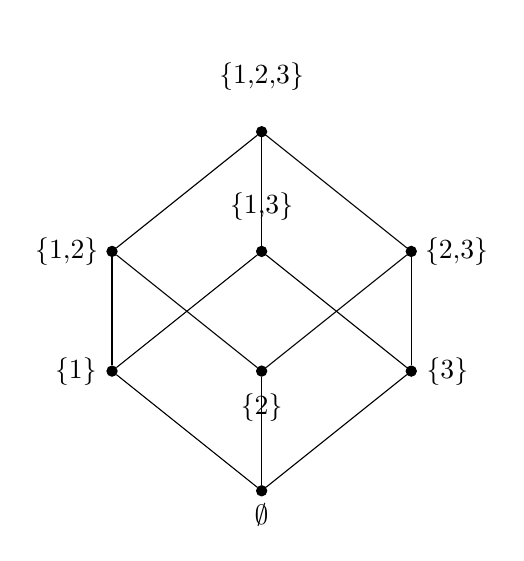
\begin{tikzpicture}[every node/.style={circle,draw,inner sep=1.3pt,fill=black},
                    scale=0.95]
  % Boolean 2^3 = subsets of {1,2,3}, ordered by inclusion. Distributive.
  \node[label=below:$\emptyset$] (bot) at (0,0) {};
  \node[label=left:$\{1\}$]  (sA) at (-2,1.6) {};
  \node[label={below:$\{2\}$}]  (sB) at ( 0,1.6) {};
  \node[label=right:$\{3\}$] (sC) at ( 2,1.6) {};
  \node[label={left:$\{1{,}2\}$}]  (sAB) at (-2,3.2) {};
  \node[label={above:$\{1{,}3\}$}]  (sAC) at ( 0,3.2) {};
  \node[label={right:$\{2{,}3\}$}] (sBC) at ( 2,3.2) {};
  \node[label=above:$\{1{,}2{,}3\}$] (top) at (0,4.8) {};
  \draw (bot)--(sA); \draw (bot)--(sB); \draw (bot)--(sC);
  \draw (sA)--(sAB); \draw (sA)--(sAC);
  \draw (sB)--(sAB); \draw (sB)--(sBC);
  \draw (sC)--(sAC); \draw (sC)--(sBC);
  \draw (sAB)--(top); \draw (sAC)--(top); \draw (sBC)--(top);
\end{tikzpicture}\\[0.4em]
{\footnotesize (a) Boolean $2^3$: \emph{distributive}.}
\end{minipage}\hfill
\begin{minipage}[b]{0.50\textwidth}\centering
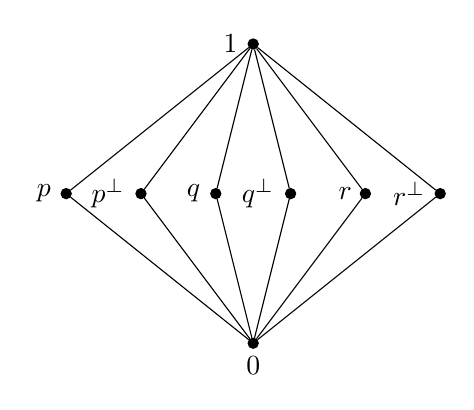
\begin{tikzpicture}[every node/.style={circle,draw,inner sep=1.3pt,fill=black},
                    scale=0.95]
  % MO3: 0 bottom, 1 top, six atoms (three complementary pairs) on one rung.
  \node[label=below:$0$] (z) at (0,0) {};
  \node[label=left:$p$]   (a)  at (-2.5,2) {};
  \node[label=left:$p^\perp$]  (ap) at (-1.5,2) {};
  \node[label={left:$q$}]  (b)  at (-0.5,2) {};
  \node[label={left:$q^\perp$}] (bp) at ( 0.5,2) {};
  \node[label=left:$r$]  (c)  at ( 1.5,2) {};
  \node[label=left:$r^\perp$] (cp) at ( 2.5,2) {};
  \node[label=left:$1$]  (o)  at (0,4) {};
  \foreach \x in {a,ap,b,bp,c,cp}{\draw (z)--(\x); \draw (\x)--(o);}
\end{tikzpicture}\\[0.4em]
{\footnotesize (b) $\mathrm{MO}_3$: \emph{non-distributive}.}
\end{minipage}
\caption{Hasse diagrams (edges are covering relations). In the Boolean
cube~(a), each singleton lies below the \emph{two} pairs that contain it;
those four-cycles are exactly distributivity, and complementation
$\{i\}\mapsto\{j,k\}$ matches the geometry. In $\mathrm{MO}_3$~(b) every
non-trivial element is \emph{both} an atom and a coatom: the lattice has
height~$3$, the three complementary pairs $(p,p^\perp),(q,q^\perp),
(r,r^\perp)$ share only $0$ and $1$, and any two distinct atoms have meet
$0$ and join $1$. Distributivity fails at once:
$p\wedge(q\vee r)=p\wedge 1=p$, but $(p\wedge q)\vee(p\wedge r)=0\vee 0=0$.
The six atoms being pairwise meet-zero is what forces
$s(p)+s(q)+s(r)\le 1$ on any extending charge, which $s\equiv\tfrac12$
violates. Structure verified in
\texttt{verification/mo3\_extension.py}.}
\label{fig:hasse}
\end{figure}

\paragraph{The concrete/non-concrete boundary is not where the gap
closes.}
A set-representable OMP $(P, L)$ requires only closure under
complement and under \emph{disjoint} union
(Bure\v{s}ov\'{a}--Pt\'{a}k~\cite{BuresovaPtak2024}, Def.~1.1);
closure under intersection is \emph{not} required --- it would force
$L$ to be a field of sets, hence Boolean.  The lattice meet $a \wedge
b$ is the greatest $L$-member contained in $A \cap B$, so $a \wedge b
\subseteq A \cap B$ with equality iff $A \cap B \in L$.  Hence
orthogonality ($A \cap B = \varnothing$) implies meet-zero always, but
\textbf{meet-zero does not imply orthogonality} for incompatible
pairs.  The smallest witness is $\mathrm{MO}_2$, the concrete logic on
$P = \{1,2,3,4\}$ with
$L = \{\varnothing, \{1,2\}, \{3,4\}, \{1,3\}, \{2,4\}, P\}$: there
$\{1,2\} \wedge \{1,3\} = 0$ while $\{1,2\} \cap \{1,3\} = \{1\} \neq
\varnothing$.  Crucially, $\mathrm{MO}_3$ \emph{itself is concrete}
(it carries $2^3$ ordering two-valued states, hence is
set-representable by Gudder's representation theorem for concrete
logics --- a concrete logic is exactly an OMP with an order-determining
set of two-valued states~\cite{PtakPulmannova1991}), so the flagship ``meet-zero $\neq$ orthogonal'' example above
is a concrete logic.  The boundary that matters is therefore not
concrete versus non-concrete but a \emph{richness} / atomicity
condition: meet-zero coincides with orthogonality iff every nonempty
$A \cap B$ contains a nonzero member of $L$ (sufficient: all singletons
lie in $L$).  This property has no established standard name (its
cousins --- Jauch--Piron, Tkadlec ``regional,''
Bure\v{s}ov\'{a}--Pt\'{a}k ``point-distinguishing'' --- are all
distinct).  (Terminology trap: $\mathrm{MO}_3$'s celebrated
non-representability is von~Neumann \emph{coordinatisation} --- failure
to be a subspace lattice of a projective geometry --- a different
notion from set-representability.)

\paragraph{Status of the extension axis.}
For \emph{rich} concrete OMLs (singletons in $L$, or the weaker
intersection-richness above) meet-zero coincides with orthogonality,
and the extension axis reduces to the classical marginal /
Pitowsky non-contextuality problem.  For \emph{non-rich} concrete OMLs
($\mathrm{MO}_2$, $\mathrm{MO}_3$) and non-concrete OMLs ($L(H)$) the
meet-zero/orthogonal gap is non-empty, and the extension axis is
strictly stronger and can fail universally.  In the \emph{finite} case
it is a decidable linear program, not a structurally resistant
frontier.  The \emph{infinite} case --- $L(H)$, to which the finite
counterexample does not directly speak --- is resolved for normal
states by the clustering argument of \S\ref{sec:lh} below, with only
the singular states left open.

\subsection{The infinite extension case for $L(H)$}
\label{sec:lh}

For $L(H)$ with $\dim H = \infty$ the extension axis admits a decisive
finite-dimensional argument, sharper than the $\mathrm{MO}_3$ linear
program.  Fix a $2$-dimensional subspace $e \subset H$.  For any line
$p \subset e$, its perpendicular $p^\perp \subset e$ satisfies
$p \perp p^\perp$ and $p \vee p^\perp = e$, so orthoadditivity gives
\begin{equation}\label{eq:lh-pair}
  s(p) + s(p^\perp) = s(e).
\end{equation}
Choose $k$ distinct lines $p_1, \dots, p_k \subset e$ in general
position, so that the $2k$ lines $\{p_i, p_i^\perp\}$ are pairwise
distinct.  Distinct lines meet only at $0$, hence are pairwise
meet-zero, so $h$ sends them to $2k$ pairwise-disjoint clopens.  A
finitely additive charge extending $\mu(h(a)) = s(a)$ must therefore
satisfy, using~\eqref{eq:lh-pair},
\begin{equation}\label{eq:lh-bound}
  \sum_{i=1}^{k} \bigl[s(p_i) + s(p_i^\perp)\bigr] = k\, s(e) \leq 1
  \qquad\text{for every } k \geq 1.
\end{equation}
If $s(e) > 0$, taking $k > 1/s(e)$ violates~\eqref{eq:lh-bound}.  Hence:

\begin{proposition}\label{prop:lh}
Any state $s$ on $L(H)$ with $s(e) > 0$ for even one finite-dimensional
$e$ fails to extend to a charge on the full clopen algebra of
$S_0(L(H))$.  In particular no normal (Gleason) state extends.  The
argument uses only orthoadditivity on lines in a single $2$-plane;
$\sigma$-completeness of the lattice is irrelevant.
\end{proposition}

Every normal state $s = \tr(\rho\,\cdot)$ has $s(e) > 0$ for some $2$-dim
$e$ (as $\rho \neq 0$), so Proposition~\ref{prop:lh} kills the entire
$\sigma$-additive (Gleason) state space.  This answers the infinite
extension question for the physically central states, and answers
``does $\sigma$-completeness change it?'' in the negative.

The only states the argument does \emph{not} reach are the
\emph{singular} ones: $s(e) = 0$ for every finite-dimensional $e$, where
the bound~\eqref{eq:lh-bound} is vacuous.  These exist (take $H$
separable) --- e.g.\ the ultrafilter vector state
$s(a) = \lim_\omega \langle a e_n, e_n\rangle$ for a free ultrafilter
$\omega$ and an orthonormal basis $(e_n)$, or any pullback of a state on
the Calkin algebra $B(H)/K(H)$.  Moreover, lifting a lattice state to a
bounded functional $\varphi$ on $B(H)$ by Mackey--Gleason /
Bunce--Wright~\cite{BunceWright1992, Christensen1982} (valid as $B(H)$
has no type $\mathrm{I}_2$ summand), the Takesaki normal/singular
decomposition $\varphi = \varphi_n + \varphi_s$ with both parts
positive~\cite{Takesaki1979} writes
$B(H)^* = (\text{trace class}) \oplus K(H)^\perp$ --- where the singular
part $\varphi_s$ \emph{annihilates the compacts} $K(H)$ (a statement at
the level of $\varphi$, after the lift, not of the bare lattice state).
A finite-rank projection $e$ then has $s(e) = \tr(\rho\, e)$, and
$s(e) = 0$ for all finite-dim $e$ forces $\rho = 0$ (taking $e$ rank-one
gives $\langle \rho \xi, \xi\rangle = 0$ for all $\xi$).  So a state is
\emph{either} detected by some finite-rank projection (killed by
Proposition~\ref{prop:lh}) \emph{or} purely singular --- a clean
dichotomy with no third class (the decomposition being unique).  The
density $\varphi_n = \tr(\rho\,\cdot)$ is named by predual duality
$B(H)_* = $ trace class, \emph{not} by Gleason.  Whether a singular orthoadditive state
extends is the open residue; there the relevant meet-zero families are
infinite-dimensional subspaces with trivial intersection, and
$\sigma$-additivity \emph{of the state} (not of the lattice) is what
bites.

The hinge --- and the first thing to settle before deciding whether this
residue is genuinely more tractable than the descent residue
(\S\ref{sec:assessment}) --- is whether the singular obstruction is
reached with \emph{finite} or \emph{countable} meet-zero families.  The
normal-state argument (Proposition~\ref{prop:lh}) is finitary: $k$ lines,
$k$ arbitrary but finite, and the bound is violated at finite $k$.  This
is why it needs no $\sigma$-duality and dodges the statability wall of
\S\ref{sec:assessment}.  But the phrase ``$\sigma$-additivity of the
state is what bites'' suggests the singular obstruction may instead
require a \emph{countable} family of infinite-dimensional subspaces ---
in which case it is \emph{not} cleanly finitary and does not obviously
dodge that wall.  If the obstruction is finite, the singular case is a
self-contained operator-algebra question (Calkin / Bunce--Wright machinery)
settleable ahead of the descent residue; if countable, it is entangled
with the same finitary-to-$\sigma$ bridge and is not clearly the easier
of the two.  Settling \emph{which} is the concrete next step; it is
mathematical work, not yet done here.  (Proposition~\ref{prop:lh} is the proof; the inequality is
instance-checked --- finitely many lines in $\mathbb{R}^2$, the charge
LP infeasible once $k\,s(e) > 1$ --- by
\texttt{verification/lh\_infinite\_extension.py}, which does not itself
touch the infinite-dimensional $S_0(L(H))$.  The singular/normal
dichotomy is hand-verified --- foundations cited with hypotheses
checked, gluing checked by hand --- in
\texttt{verification/lh\_singular\_dichotomy.md}.)

\paragraph{Descent.}
$\sigma$-additivity of the state governs descent, not extension.
Even once $\mu$ extends to a measure $\hat\mu$ on $S_0(A)$, the
\emph{descent} question --- whether $\hat\mu$ concentrates on the
``physical'' points --- changes character:
\begin{description}[style=nextline, font=\normalfont\bfseries,
    labelwidth=2.5cm, leftmargin=3cm]
  \item[Boolean]
    Does $\hat\mu$ concentrate on $\pure(\Omega)$?  If and only if
    the charges are $\sigma$-additive.  The choice of realisation
    space $\Omega$ is unconstrained.
  \item[OML]
    Does $\hat\mu$ concentrate on $P(A)$?  Here $P(A)$ is part of
    the structure, not a free choice.  The Kochen--Specker
    obstruction~\cite{KochenSpecker1967} prevents simultaneous
    realisation of all filters; the Bub--Clifton
    theorem~\cite{BubClifton1996} shows that the state determines
    a maximal Boolean subalgebra of definite values.
\end{description}
In the OML setting, the algebra and state \emph{together}
constrain which filters are ``realised.''  Descent is not a
geometric commitment but a structural consequence.

\begin{remark}[Decomposition lives on the descent axis]
De Simone--Navara~\cite{DeSimoneNavara2001} decompose OMP states as
$s = s_\sigma + s_{\mathrm{wpfa}}$ (a $\sigma$-additive part and a
weakly purely finitely additive part), the orthomodular analogue of
Yosida--Hewitt.  By the axis split above, the wpfa component governs
the \emph{descent} axis --- it is the analogue of the purely finitely
additive part $\ell_p$ in the Boolean case --- and \emph{not} the
extension axis.  A natural-looking conjecture, ``$s$ extends iff
$s_{\mathrm{wpfa}} = 0$,'' is therefore mis-targeted: vanishing of
$s_{\mathrm{wpfa}}$ concerns whether the (already $\sigma$-additive)
state's measure concentrates on $P(A)$, while extension is blocked by
non-distributivity regardless of the wpfa component.  The
decomposition theory and the extension problem live on different
axes.

A caveat compounds this.  The McDonald--Bimb\'{o}
duality~\cite{McDonaldBimbo2023} is \emph{finitary}: the identity
$h(\bigvee_n a_n) = (\bigcup_n h(a_n))^{\perp\perp}$ holds for finite
joins but fails in general for countable joins, since finitary OML
homomorphisms need not preserve infinite suprema.  Making even the
descent argument rigorous --- the analogue of Paper~I's
``$\sigma$-additivity $\Leftrightarrow$ concentration'' --- requires
$\sigma$-completeness and continuity hypotheses the 2023 duality does
not supply, and is itself open.
\end{remark}

\paragraph{The finitary-to-$\sigma$ bridge: open, with three named
routes blocked.}
Paper~I's descent runs on a \emph{Loomis--Sikorski} engine:
$\sigma$-additive measures on the Stone space correspond to
$\sigma$-homomorphisms off the ideal points, which is what makes
``$\sigma$-additive $\Leftrightarrow$ concentrates on
$\pure(\Omega)$'' go through.  The OML descent question is whether
that engine has an OML analogue --- whether a $\sigma$-complete OML
admits a Loomis--Sikorski representation (quotient of a
$\sigma$-tribe of sets by a $\sigma$-ideal) or a countable-join-
preserving $\sigma$-Stone duality.  The literature settles only the
known \emph{routes}, all of which are blocked.
\begin{enumerate}[label=(\roman*), noitemsep]
  \item \textbf{RDP / effect-algebra route --- blocked.}
    Loomis--Sikorski holds for $\sigma$-complete MV-algebras
    (Dvure\v{c}enskij~\cite{Dvurecenskij2000}) and for monotone
    $\sigma$-complete effect algebras \emph{with} the Riesz
    Decomposition Property (RDP)~\cite{Dvurecenskij2005}.  But a
    lattice effect algebra has RDP iff it is an MV-algebra
    (Rie\v{c}anov\'{a}; Paseka), and an OML that is an MV-algebra ---
    all pairs compatible --- is Boolean (Kalmbach~\cite{Kalmbach1983}).
    So $\text{OML} + \text{RDP} \Leftrightarrow \text{Boolean}$: the
    RDP machinery has no non-Boolean OML to act on.
  \item \textbf{MacNeille-completion route --- blocked.}
    Harding~\cite{Harding1991} shows the MacNeille completion of an
    OML need not be orthomodular, so one cannot complete to absorb
    countable joins.
  \item \textbf{$\sigma$-Stone-duality route --- none exists.}
    McDonald--Bimb\'{o} is irreducibly finitary; Freytes' equational
    theory of $\sigma$-complete OMLs~\cite{Freytes2020} supplies no
    set/tribe representation.
\end{enumerate}
A concentration statement needs a point space, which a general OML
may lack (Greechie stateless lattices are non-concrete).  But that is
a red herring for the live case: $L(H)$ is non-concrete yet Gleason
hands it a clean lattice measure (the non-concreteness is no obstacle
there), and $\mathrm{MO}_3$ is concrete.  The genuinely open class is
\textbf{concrete, non-Boolean, infinite $\sigma$-OMLs}, where the
non-concreteness obstruction is absent and
the RDP argument blocks only one route.  No impossibility theorem is
known for this class; the contribution here is the map of dead routes,
which sharpens ``needs a new idea'' into ``needs a representation
bypassing all three.''

\paragraph{What is at stake: relational probability without realizations.}
The descent residue carries a motivation beyond technical
completeness.  Paper~I's finding was that \emph{realization} ---
which points are ``real'' --- is structure added on top of a coherent
assignment, not forced by it.  In the McDonald--Bimb\'{o} setting,
realization is concentration on the dual points $P(A) \subseteq
S_0(A)$.  A construction of $\sigma$-additive probability on a
non-distributive OML \emph{that does not pass through such a
concentration} would be probability built from the entailment relation
alone --- a relational, point-free probability, the non-Boolean analogue
of the localic (pointless) measures distributivity already permits.

Two cautions keep this honest.  First, the separation already
established for $L(H)$ --- a $\sigma$-additive measure exists on the
lattice ($\text{PR}_{\text{lat}}$, by Gleason) while no measure
concentrates on the dual points ($\text{PR}_{\text{dual}}$ fails,
\S\ref{sec:lh}) --- shows a lattice measure \emph{need not descend to
the McDonald--Bimb\'{o} points}.  But it does \emph{not} exhibit
point-free probability: ``point'' is overloaded.  Gleason removes the
\emph{dual} points $P(A)$ while resting entirely on the \emph{Hilbert}
points (the rays of $H$, from which the density $\rho$ in
$s = \tr(\rho\,\cdot)$ is built); indeed Gleason is a \emph{representation}
theorem, reducing every lattice state to that point datum.  So $L(H)$
witnesses the separation, not point-freeness, and cannot serve as the
existence proof we want.  Second, Gleason fires only because $H$ is
present; for a general OML there is no such theorem.  Hence a genuinely
point-free construction must be built, not borrowed --- and the only
route to it is exactly the missing $\sigma$-OML representation of the
route-map above.  This is the substantive reason to chase residue~\#2:
it is the engine for relational probability without realizations, and ---
since $L(H)$/Gleason does not supply that witness --- the \emph{only}
candidate engine, not a redundant one.

\paragraph{Two grades of probabilistic realism.}
The two axes, re-expressed in the EA/PR/VDR vocabulary of
Paper~II~\cite{MahonPaperII2026}, split \emph{probabilistic realism}
(PR) into two grades that the Boolean case fuses and non-distributivity
separates --- the same extension/descent split, named in the realism
language, not a new construction.
\begin{description}[style=nextline, font=\normalfont\bfseries,
    labelwidth=2.2cm, leftmargin=2.6cm]
  \item[$\text{PR}_{\text{lat}}$]
    A $\sigma$-additive measure on the \emph{lattice} $A$ agreeing with
    $s$. For $L(H)$, $\dim H \geq 3$, Gleason supplies this for every
    $\sigma$-additive state.
  \item[$\text{PR}_{\text{dual}}$]
    A $\sigma$-additive Borel measure $\hat\mu$ on the \emph{dual}
    $S_0(A)$ with $\hat\mu(h(a)) = s(a)$ concentrating on the physical
    points, $\hat\mu(P(A)) = 1$ --- extension (\S\ref{sec:problem})
    followed by descent.
\end{description}
The relation between the two grades is a \emph{witnessed
one-directional separation}, not a proven nesting.  $L(H)$ normal states
\emph{separate} them: they clear $\text{PR}_{\text{lat}}$ (Gleason) and
fail $\text{PR}_{\text{dual}}$ (\S\ref{sec:lh}: no charge on $S_0(L(H))$
exists, a fortiori none concentrating).  The reverse inclusion
$\text{PR}_{\text{dual}} \Rightarrow \text{PR}_{\text{lat}}$ is
\emph{not} free: restricting a dual measure $\hat\mu$ to the
$\perp$-stable clopens recovers $s$ only as a \emph{finitely}
orthoadditive state, whereas $\text{PR}_{\text{lat}}$ needs
$\sigma$-additivity on the lattice, $s(\bigvee_n a_n) = \sum_n s(a_n)$.
The gap is $\hat\mu(D)$, $D = h(\bigvee_n a_n) \setminus \bigcup_n
h(a_n)$, and concentration on $P(A)$ does \emph{not} force $\hat\mu(D) =
0$: $D$ contains \emph{principal} filters (e.g.\ $\uparrow\!p$ with
$p = \mathrm{span}(v)$, $v$ of infinite support, $a_n = \mathrm{span}(e_n)$:
$p \leq \bigvee_n a_n$ but $p \not\leq a_n$ for all $n$).  So
$\text{PR}_{\text{dual}} \Rightarrow \text{PR}_{\text{lat}}$ requires an
extra $\sigma$-continuity hypothesis ($\hat\mu$ null on countable-join
defects) that the finitary McDonald--Bimb\'{o} duality does not supply
--- the \emph{same} finitary wall flagged above (verified against the
primary source, \texttt{verification/mb\_primeness\_check.md}).  What
\emph{is} established is the separation, and it lets one assert
\emph{both} grades at once --- Gleason clears $\text{PR}_{\text{lat}}$
for $L(H)$ while $\text{PR}_{\text{dual}}$ fails --- without suppressing
either.  In the Boolean case the two grades coincide (Stone gives
$\hat\mu$ unconditionally; descent $\Leftrightarrow$ $\sigma$-additivity),
which is why Paper~II could write a single PR.  The distinction is
philosophically neutral: a Born-rule realist reads off
$\text{PR}_{\text{lat}}$, a relational realist $\text{PR}_{\text{dual}}$,
a constructive empiricist EA.

What is \emph{not} established is that descent does any work independent
of extension.  Every known $\text{PR}_{\text{dual}}$ failure is an
extension failure; in finite dimensions descent is vacuous (the only
non-principal point is the improper filter, already null by $s(0)=0$ ---
verified, \texttt{verification/pr\_dual\_inhabitation.py}, where
$\text{PR}_{\text{dual}}$ on $\mathrm{MO}_2$ collapses to the extension
LP).  The descent half can be strictly weaker than extension only in
infinite dimensions, where free non-principal filters can carry mass ---
exactly where the finitary-to-$\sigma$ bridge above fails.  Hence the
open question: \emph{is there a $\sigma$-OML regime in which descent is
both statable and strictly weaker than extension --- a non-distributive
OML and state that extends to a charge on $S_0(A)$ but fails to
concentrate on $P(A)$?}  The only candidate is the singular-state sliver
of \S\ref{sec:lh}, which runs into the same statability wall.  Until such
a witness exists, $\text{PR}_{\text{lat}}/\text{PR}_{\text{dual}}$ is a
witnessed one-directional \emph{separation} ($L(H)$ normal states clear
$\text{PR}_{\text{lat}}$, fail $\text{PR}_{\text{dual}}$) --- \emph{not} a
proven nesting, since $\text{PR}_{\text{dual}} \Rightarrow
\text{PR}_{\text{lat}}$ needs the same $\sigma$-continuity hypothesis the
finitary duality withholds --- with the descent half not yet shown
independent: a vocabulary refinement, not a new theorem.

% ==================================================================
\section{What is known}
\label{sec:known}
% ==================================================================

In the Boolean case, the Kelley--Vladimirov--Pt\'{a}k
characterisation (Fremlin,
Theorem~391D~\cite{Fremlin3}) gives a complete algebraic answer:

\begin{theorem}[KVP]\label{thm:kvp}
A Boolean algebra $B$ carries a strictly positive
$\sigma$-additive measure if and only if $B$ is
\begin{enumerate}[label=(\alph*), noitemsep]
  \item Dedekind $\sigma$-complete,
  \item weakly $(\sigma,\infty)$-distributive, and
  \item chargeable (carries a strictly positive finitely additive
    measure).
\end{enumerate}
\end{theorem}

Each condition is algebraic and non-trivially constraining.  For
OMLs, the analogues fail or degenerate:
\begin{enumerate}[label=(\alph*), noitemsep]
  \item Dedekind $\sigma$-completeness makes sense but is very
    strong.
  \item Weak $(\sigma,\infty)$-distributivity has no clean OML
    analogue --- the definition relies on distributivity of
    $\bigwedge$ over $\bigvee$, which may fail orthomodularly.
  \item Chargeability has no known structural characterisation on
    OMLs; the existence of a strictly positive finitely additive
    measure cannot be read off from the lattice structure.
\end{enumerate}

The positive results that do exist for OMLs all require algebraic
structure rich enough to approximate Hilbert-space geometry:
\begin{description}[style=nextline, font=\normalfont\bfseries,
    labelwidth=4cm, leftmargin=4.5cm]
  \item[Gleason~\cite{Gleason1957}]
    $A = L(H)$, $\dim H \geq 3$.  Every state has the
    form~\eqref{eq:gleason}; $\sigma$-additivity \emph{on the lattice}
    is automatic (this is lattice-level, not dual-space extension ---
    cf.\ \S\ref{sec:lh}).
  \item[Bunce--Wright~\cite{BunceWright1992}]
    $A$ the projection lattice of a JBW-algebra.
    $\sigma$-additivity via operator-algebraic structure.
  \item[Chetcuti--Dvure\v{c}enskij~\cite{ChetcutiDvurecenskij2005}]
    Lattice effect algebras with completeness conditions close to
    von~Neumann algebras.
\end{description}

The obstructive results show that the Boolean extension machinery
cannot be transplanted:
\begin{description}[style=nextline, font=\normalfont\bfseries,
    labelwidth=4cm, leftmargin=4.5cm]
  \item[Pt\'{a}k--Pulmannov\'{a}~\cite{PtakPulmannova1991}]
    If every unital subadditive measure on an orthomodular poset is
    a state, the poset must be Boolean.  This is the structural
    reason no KVP analogue exists for OMLs: conditions strong enough
    to force $\sigma$-additivity collapse the lattice back to a
    Boolean algebra.
  \item[Navara~\cite{Navara1992}]
    Regularity does \emph{not} force $\sigma$-additivity on general
    orthomodular posets.  The B\'{e}aver--Cook result is special to
    von~Neumann algebras.
  \item[Pt\'{a}k~\cite{Ptak1987}]
    Exotic OML state spaces exist; the obstruction is combinatorial
    (Greechie pasting), not from the centre.
\end{description}

Recent incremental work confirms the field is active but no one
has found the right condition:
Vor\'{a}\v{c}ek--Pt\'{a}k~\cite{VoracekPtak2023} study signed
measures on orthomodular posets;
Bure\v{s}ov\'{a}--Pt\'{a}k~\cite{BuresovaPtak2023} investigate
variations on regularity conditions; De~Simone--Navara study
Yosida--Hewitt-type decompositions for orthomodular posets.

For the \emph{$\sigma$-additivity / descent} side, the gap between
``too weak'' (allows non-$\sigma$-additive states) and ``too
strong'' (collapses to Boolean) appears structurally robust ---
this is the part where further reading has not produced the answer.
(This robustness is about the descent axis; the extension axis is
classical, per \S\ref{sec:problem}.)

\paragraph{Prior art on point-free / contextual quantum probability,
and where the gap sits.}
The point-free and directed-context constructions of quantum
probability in the literature each land on one side of a single line ---
the $\sigma$-additivity-on-a-non-distributive-structure line --- and
none crosses it.
\begin{description}[style=nextline, font=\normalfont\bfseries,
    labelwidth=3cm, leftmargin=3.4cm]
  \item[Gleason tradition]
    Varadarajan, Kalmbach, Pt\'{a}k--Pulmannov\'{a}: $\sigma$-additive
    measures on a genuinely non-distributive OML, but real-valued on a
    \emph{fixed} lattice --- not point-free and not built from a
    directed observation system.
  \item[D\"{o}ring 2009]
    \cite{Doering2009measures} builds measures point-free on the
    spectral presheaf, indexed over the directed poset of abelian
    subalgebras --- but they are provably only \emph{finitely additive}
    (a consequence of linearity of the underlying state), and live on
    the distributive Heyting algebra of clopen subobjects.
  \item[Heunen--Landsman--Spitters]
    \cite{HeunenLandsmanSpitters2009, HeunenLandsmanSpitters2011}
    (Bohrification) build point-free quantum probability over the
    directed poset of commutative subalgebras, and their internal
    valuation \emph{is} $\sigma$-additive --- it is a \emph{continuous}
    (Scott-continuous) valuation, $\mu(\bigvee_i U_i) = \bigvee_i
    \mu(U_i)$ on directed families. But it factors through an internally
    \emph{distributive} locale: externally (their Def.~for Rickart
    $C^*$-algebras) the measure is $\sigma$-additive only \emph{on each
    countably complete Boolean sublattice} of $\mathrm{Proj}(A)$, glued
    over the context poset. Non-distributivity is tamed by retreat to
    commutative contexts, not carried natively.
  \item[Localic valuations]
    Vickers, Simpson, Coquand--Spitters: point-free $\sigma$-additive
    (Scott-continuous) probability, but valuations are defined on
    \emph{frames}, distributive by definition; no orthomodular analogue
    exists in this tradition.
  \item[OML Stone dualities]
    Two finitary dualities for OMLs exist: McDonald--Bimb\'{o}
    \cite{McDonaldBimbo2023} (filter spectrum, used here) and the
    spectral-presheaf duality of Cannon and
    D\"{o}ring~\cite{Cannon2013}. Both are \emph{purely structural} ---
    neither carries a measure, state, or valuation on the
    non-distributive dual, and neither has a countable-join-respecting
    ($\sigma$-) version.
\end{description}
The descent residue is exactly the unoccupied conjunction: a
\emph{point-free}, \emph{$\sigma$-additive} measure on a \emph{natively
non-distributive} OML, built from the directed observation system, with
realization (concentration on $P(A)$) as separable structure. D\"{o}ring
gives up $\sigma$-additivity; Bohrification and the localic tradition
give up native non-distributivity (retreating to distributive
contexts/locales); the Gleason tradition gives up point-freeness. The
McDonald--Bimb\'{o} filter route is chosen over Cannon--D\"{o}ring
precisely because it carries the principal filters $P(A)$ as explicit
structure --- the realization datum the programme treats as separable.
The contribution, were it to clear its bar, is therefore the
$\sigma$-OML representation itself together with the
collective-exhaustion extension mechanism delivering
$\sigma$-additivity point-free where D\"{o}ring's reaches only finite
additivity; the \emph{directed-context-yields-non-distributivity} idea
on its own is \emph{not} new (it is the shape of both Bohrification and,
purely structurally, the colimit-over-Boolean-contexts generation of
OMLs).

All known exotic OML state spaces are built by \textbf{Greechie
pasting}~\cite{Wilce2009, Shultz1974, Ptak1987}.  Progress on the
descent residue likely requires either:
\begin{enumerate}[label=(\alph*)]
  \item a new pasting technique that controls $\sigma$-additivity,
    or
  \item an approach that bypasses the state space entirely (e.g.,
    categorical or
    topos-theoretic~\cite{DoeringIsham2008}).
\end{enumerate}

% ==================================================================
\section{Assessment}
\label{sec:assessment}
% ==================================================================

Question~\ref{q:extension}, once split into its two axes, is not a
single open problem but a settled axis and an open one.

\medskip\noindent
\textbf{Extension axis: largely settled, and partly degenerate.}
This is the classical Boolean extension
problem~\cite{HornTarski1948} / Pitowsky polytope
feasibility~\cite{Pitowsky1989}.  Because $h$ preserves meets, it
is governed by the gap between meet-zero and orthogonality, which
is non-empty whenever the concrete representation is non-rich (and a
fortiori in any non-distributive OML).  In the finite case it is a
decidable linear program; it can fail for \emph{every} state
($\mathrm{MO}_3$).  This is not a structurally resistant frontier
and does not require a new idea.  Two earlier framings of this axis
were mistaken.  (i)~``The Pt\'{a}k--Pulmannov\'{a} frontier needing a
new idea'' --- Pt\'{a}k--Pulmannov\'{a}~\cite{PtakPulmannova1994}
concerns the \emph{supply} of valuations (a unital set forces
Boolean), not whether a given state extends, and extension is in
any case strictly stronger than the valuation condition.
(ii)~``Concrete OMLs reduce the axis to Pitowsky non-contextuality
because meet $=$ intersection'' --- false: concreteness requires only
disjoint-union closure, and $\mathrm{MO}_2$, $\mathrm{MO}_3$ are
concrete logics in which meet-zero $\neq$ orthogonality
(\S\ref{sec:problem}).  The gap closes only under a richness /
atomicity hypothesis, not under concreteness.

\medskip\noindent
\textbf{Descent axis: genuinely open, dead routes mapped.}  Whether a
measure on $S_0(A)$ concentrates on the physical points $P(A)$, and
the analogue of Paper~I's ``$\sigma$-additivity $\Leftrightarrow$
concentration,'' cannot even be stated rigorously without
$\sigma$-completeness and continuity hypotheses, because the
McDonald--Bimb\'{o} duality is finitary (the countable-join identity
fails).  The descent argument runs on a Loomis--Sikorski engine, and
the three known routes to an OML analogue are all blocked --- the
RDP / effect-algebra route ($\text{OML} + \text{RDP} \Leftrightarrow
\text{Boolean}$), the MacNeille completion (Harding), and a
$\sigma$-Stone duality (none exists; Freytes gives only an equational
theory).  But \emph{no impossibility theorem} is known for the live
class --- concrete, non-Boolean, infinite $\sigma$-OMLs.  This is the
live residue, now sharpened from ``needs a new idea'' to ``needs a
representation bypassing all three blocked routes.''

\medskip\noindent
\textbf{The infinite extension case: no normal state extends; the
singular case is the open sliver.}  For $L(H)$ with $\dim H = \infty$
the extension fails decisively for every normal state, by a clustering
argument inside a single $2$-plane (\S\ref{sec:lh}).  Fix a $2$-dim
subspace $e$; for $k$ distinct lines $p_1, \dots, p_k \subset e$, the
$2k$ lines $\{p_i, p_i^\perp\}$ are pairwise meet-zero, so a charge
forces $\sum_i [s(p_i) + s(p_i^\perp)] = k\, s(e) \leq 1$ for every $k$.
Hence any state with $s(e) > 0$ for even one finite-dim $e$ fails ---
which is every normal (Gleason) state.  $\sigma$-completeness of the
lattice is irrelevant; extension is a finitary charge condition.  The
only escapees are \emph{singular} states ($s(e) = 0$ for all finite-dim
$e$); these exist (e.g.\ ultrafilter vector states, or pullbacks of
Calkin-algebra states) and form, with the normal states, a clean
dichotomy (Takesaki normal/singular decomposition via the Bunce--Wright
lift~\cite{BunceWright1992}).  Whether a singular orthoadditive state
extends --- where the relevant meet-zero families are infinite-dim
subspaces with trivial intersection, and $\sigma$-additivity \emph{of
the state} is what bites --- is the open sliver.

\medskip\noindent
\textbf{Novelty.}\enspace The formulation via McDonald--Bimb\'{o}
duality~\cite{McDonaldBimbo2023} appears to be new; the
identification of the extension axis with classical Horn--Tarski /
Pitowsky feasibility de-mystifies it.  For $L(H)$, Gleason gives the
$\sigma$-additive measure on the \emph{lattice} $L(H)$ itself --- but
this lattice-level rigidity does \emph{not} transfer to the dual: the
clustering argument (\S\ref{sec:lh}) shows the passage to a charge on
$S_0(L(H))$ fails for every normal state.  Since extension fails there
is no dual measure $\hat\mu$ to descend, so the descent question does
not even arise for normal states on $L(H)$.

\medskip\noindent
\textbf{Status.}\enspace Extension axis: settled (finite; infinite
$L(H)$ resolved for normal states by Proposition~\ref{prop:lh}, the
singular case the open sliver).  Descent axis: open, three known routes
blocked (RDP / MacNeille / $\sigma$-Stone), no impossibility theorem.
Not a current active lead.

\medskip\noindent
\textbf{The frontier and the first concrete move.}\enspace The
computational and literature work is exhausted; what remains is human
mathematical work, in two branches that share one wall.

\begin{description}[style=nextline, font=\normalfont\bfseries,
    labelwidth=2.6cm, leftmargin=3cm]
  \item[(a)~The deep unlock]
    the $\sigma$-OML duality prerequisite (descent axis).  Build a
    Loomis--Sikorski-type representation, or a countable-join-preserving
    $\sigma$-Stone duality, for a concrete non-Boolean infinite
    $\sigma$-OML --- or prove none exists.  All three known routes are
    blocked but no impossibility theorem rules it out, so the outcome is
    binary and large: a new representation resolves the cluster, an
    impossibility result closes it (and both downstream residues) at
    once.  High ceiling, no current foothold.
  \item[(b)~The tractable special case]
    the singular-state sliver (\S\ref{sec:lh}): does a singular
    orthoadditive state on $L(H)$ extend to a charge on $S_0(L(H))$?
    A concrete operator-algebra question (Calkin, Bunce--Wright,
    Takesaki) about one specific lattice, \emph{conditionally}
    self-contained --- see the finite-vs-countable hinge below.
\end{description}

\noindent
Sequence \textbf{(b) first}, for a reason that does not depend on its
being easy: it is informative either way.  If a singular state fails to
extend, then \emph{no} state on $L(H)$ extends, so $\text{PR}_{\text{dual}}$
fails for all of $L(H)$; since the singular sliver is the only candidate
witness for ``descent does independent work'' (\S\ref{sec:assessment},
two grades), this closes the $\text{PR}_{\text{dual}}$ third-grade
question negatively --- an impossibility-flavoured closure.  If a singular
state \emph{does} extend, it is the first concrete object that extends but
may not concentrate, which hands branch~(a) its motivating example.  Either
outcome advances the cluster.

\medskip\noindent
\textbf{The hinge that gates (b).}\enspace Whether (b) is genuinely the
easier branch turns on a single fact, \emph{not yet settled}: is the
singular-extension obstruction reached with \emph{finite} or
\emph{countable} meet-zero families (\S\ref{sec:lh})?  The normal-state
result is finitary and so dodges the descent-axis statability wall; the
singular case names ``$\sigma$-additivity of the state'' as operative,
which would make it countable --- and then it is not cleanly finitary and
does not obviously dodge that wall.  Settle finite-vs-countable first: if
finite, (b) is a self-contained operator-algebra problem to attack ahead
of (a); if countable, (b) is entangled with the same finitary-to-$\sigma$
bridge as (a) and the tractability advantage evaporates.

\bibliographystyle{plain}
\bibliography{references_oml}
\end{document}
